\section{Desenvolvimento do código}
Para desenvolver o código, utilizamos o Visual Studio Code (VSCode) junto com a extensão do Platform IO. A extensão nos dá acesso à página inicial do PlatformIO. Criamos um projeto chamado "pwm\_", definimos que a placa é Espressif ESP32 Dev Module e que o framework a ser utilizado é o Arduino.

Com o projeto criado, acessamos o arquivo platformio.ini e definimos que a taxa do monitor é de 9600. Para então, irmos ao arquivo main.cpp e iniciarmos o Serial com a taxa que escolhemos na função \textit{setup}.

\begin{lstlisting}
// platformio.ini
monitor_speed = 9600

// main.cpp
void setup() {
    Serial.begin(9600);
}

\end{lstlisting}

No início do código, definimos constantes para que guardem o valor dos pinos escolhidos.

\begin{lstlisting}
#define RED 18
#define GREEN 19
#define BLUE 21
\end{lstlisting}

Em \textit{setup}, configuramos o modo dos pinos para que sejam de saída.

\begin{lstlisting}
pinMode(RED, OUTPUT);
pinMode(GREEN, OUTPUT);
pinMode(BLUE, OUTPUT);
\end{lstlisting}

Para definir a intensidade do brilho de cada LED, usamos a função \textit{analogWrite} que recebe como parâmetros o número do pino e o valor do \textit{duty cycle}, que vai de 0 até 255. O \textit{duty cycle} é a largura do pulso da onda. Para cada terminal do LED RGB, iremos usar essa função.

\begin{lstlisting}
void analogWrite(uint8_t pin, int value);
\end{lstlisting}

Escolhemos as cores amarelo, roxo e laranja para testar essa funcionalidade. Para saber os valores, visitamos o site \href{https://htmlcolorcodes.com/}{htmlcolorcodes.com} que fornece um \textit{color picker} e mostra como essa cor pode ser definida em diferentes formados, como o RGB.

\begin{figure}[H]
    \centering
    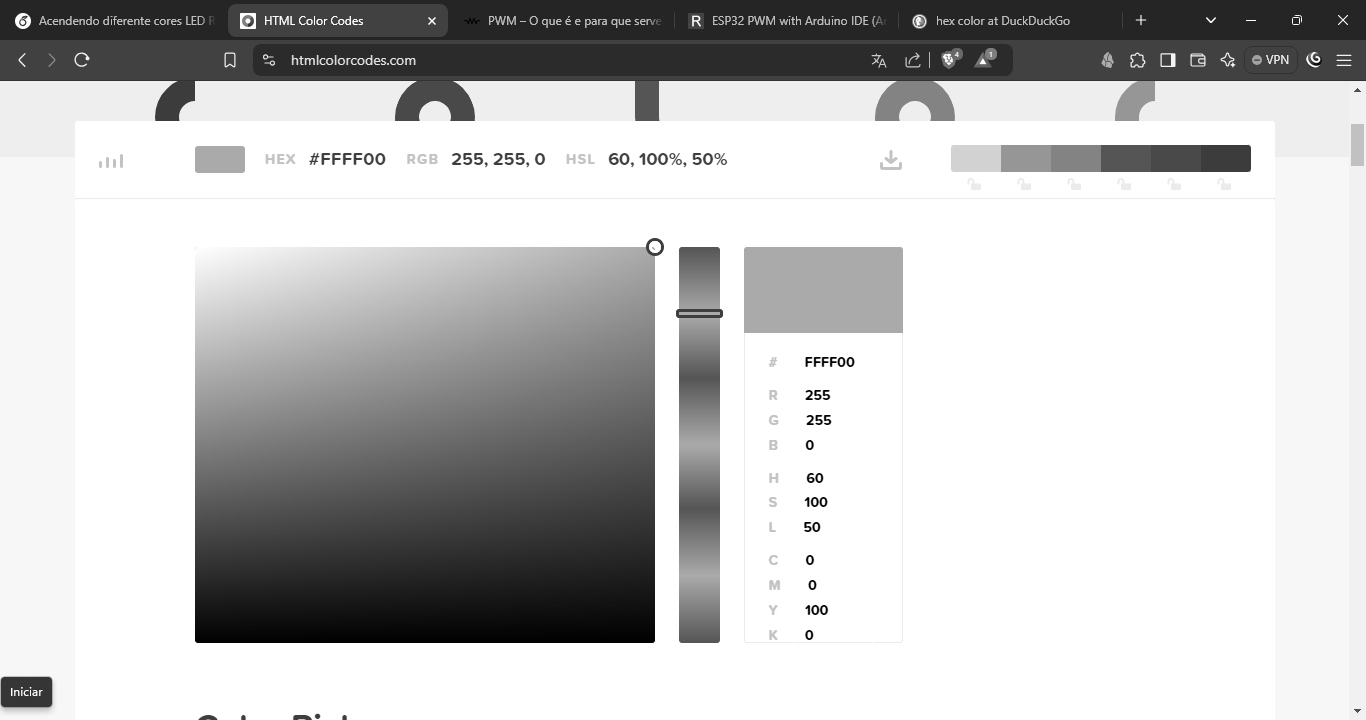
\includegraphics[width=0.5\linewidth]{img/htmlcolors.jpg}
    \caption{Site HTML Color Codes}
    \label{fig:html-color-codes-site}
\end{figure}

Recolhendo as informações e aplicando nas funções, o código fica dessa forma.

\begin{lstlisting}
void loop() {
    // yellow
    analogWrite(RED, 255);
    analogWrite(GREEN, 255);
    analogWrite(BLUE, 0);
    
    // purple
    analogWrite(RED, 158);
    analogWrite(GREEN, 10);
    analogWrite(BLUE, 149);
    
    // orange
    analogWrite(RED, 251);
    analogWrite(GREEN, 64);
    analogWrite(BLUE, 3);
}
\end{lstlisting}

Adicionamos um \textit{delay} de três segundos após cada configuração para que seja possível visualizar cada uma das cores.

\begin{lstlisting}
delay(3000);
\end{lstlisting}
